\documentclass[aspectratio=169]{beamer}

% \renewcommand{\textSupervisors}    {Supervisors}

\usetheme{vega}

\title{Forecasting the Yield Curve: An Econometric Study}
\subtitle{Financial Econometrics}
\author{Vsevolod Zaostrovsky, Ivan Cherepakhin, Artemy Sazonov}
\institute{Vega Institute Foundation}
\supervisor{Ivan P. Stankevich}
% \date{August 21 -- 28, 2022}

\begin{document}
\maketitle

\begin{frame}{The Data}
    \begin{figure}
        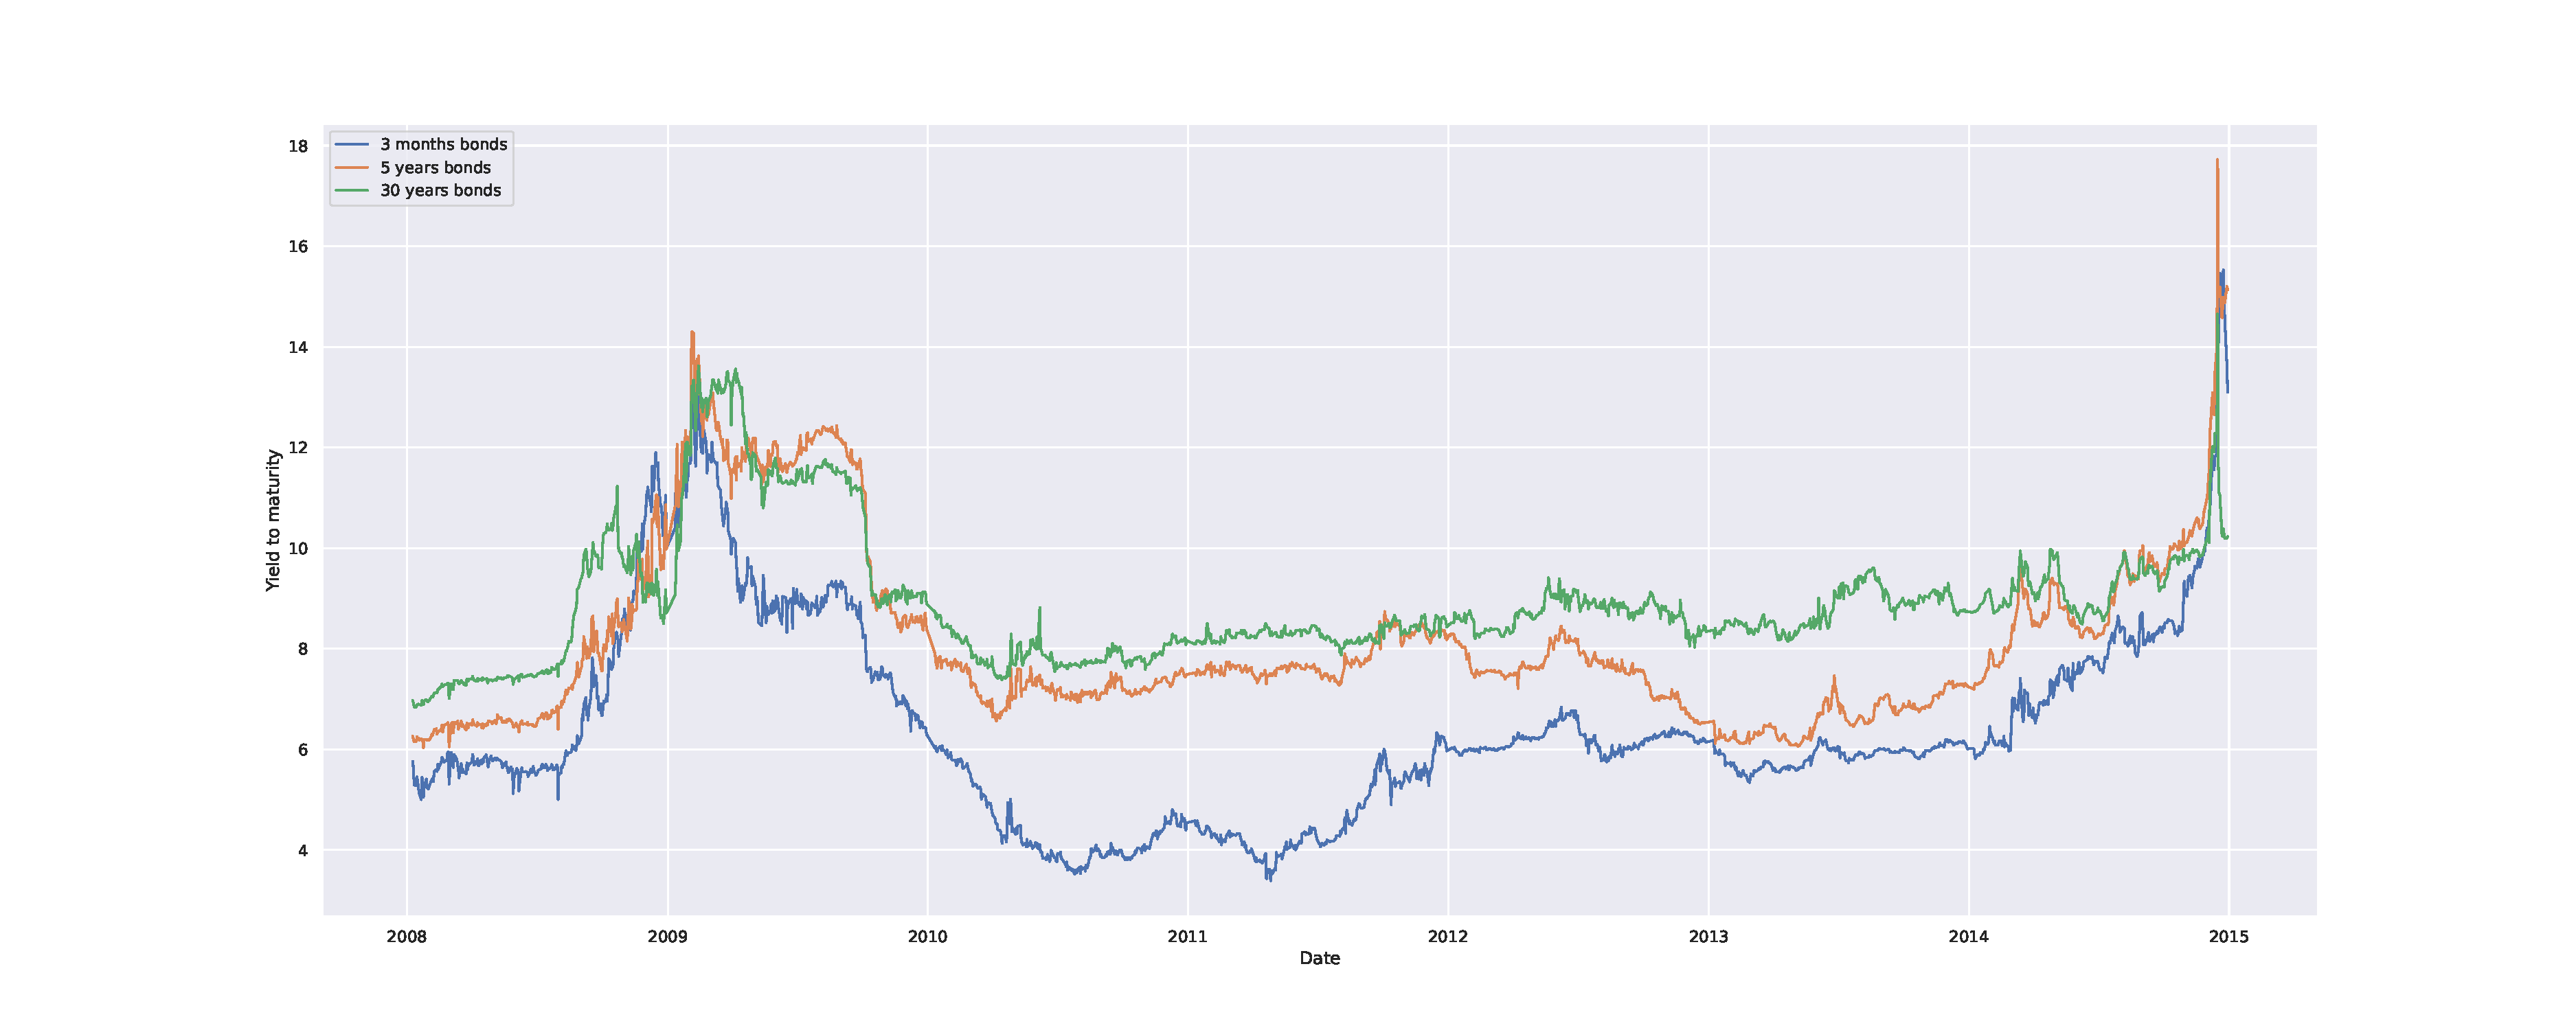
\includegraphics[scale=0.21]{fig/YTMp.pdf}
        \caption{YTM for three different bonds}
        \label{fig:YTMp}
    \end{figure}
\end{frame}

    \begin{frame}{The Yield Curve}
        \begin{figure}
            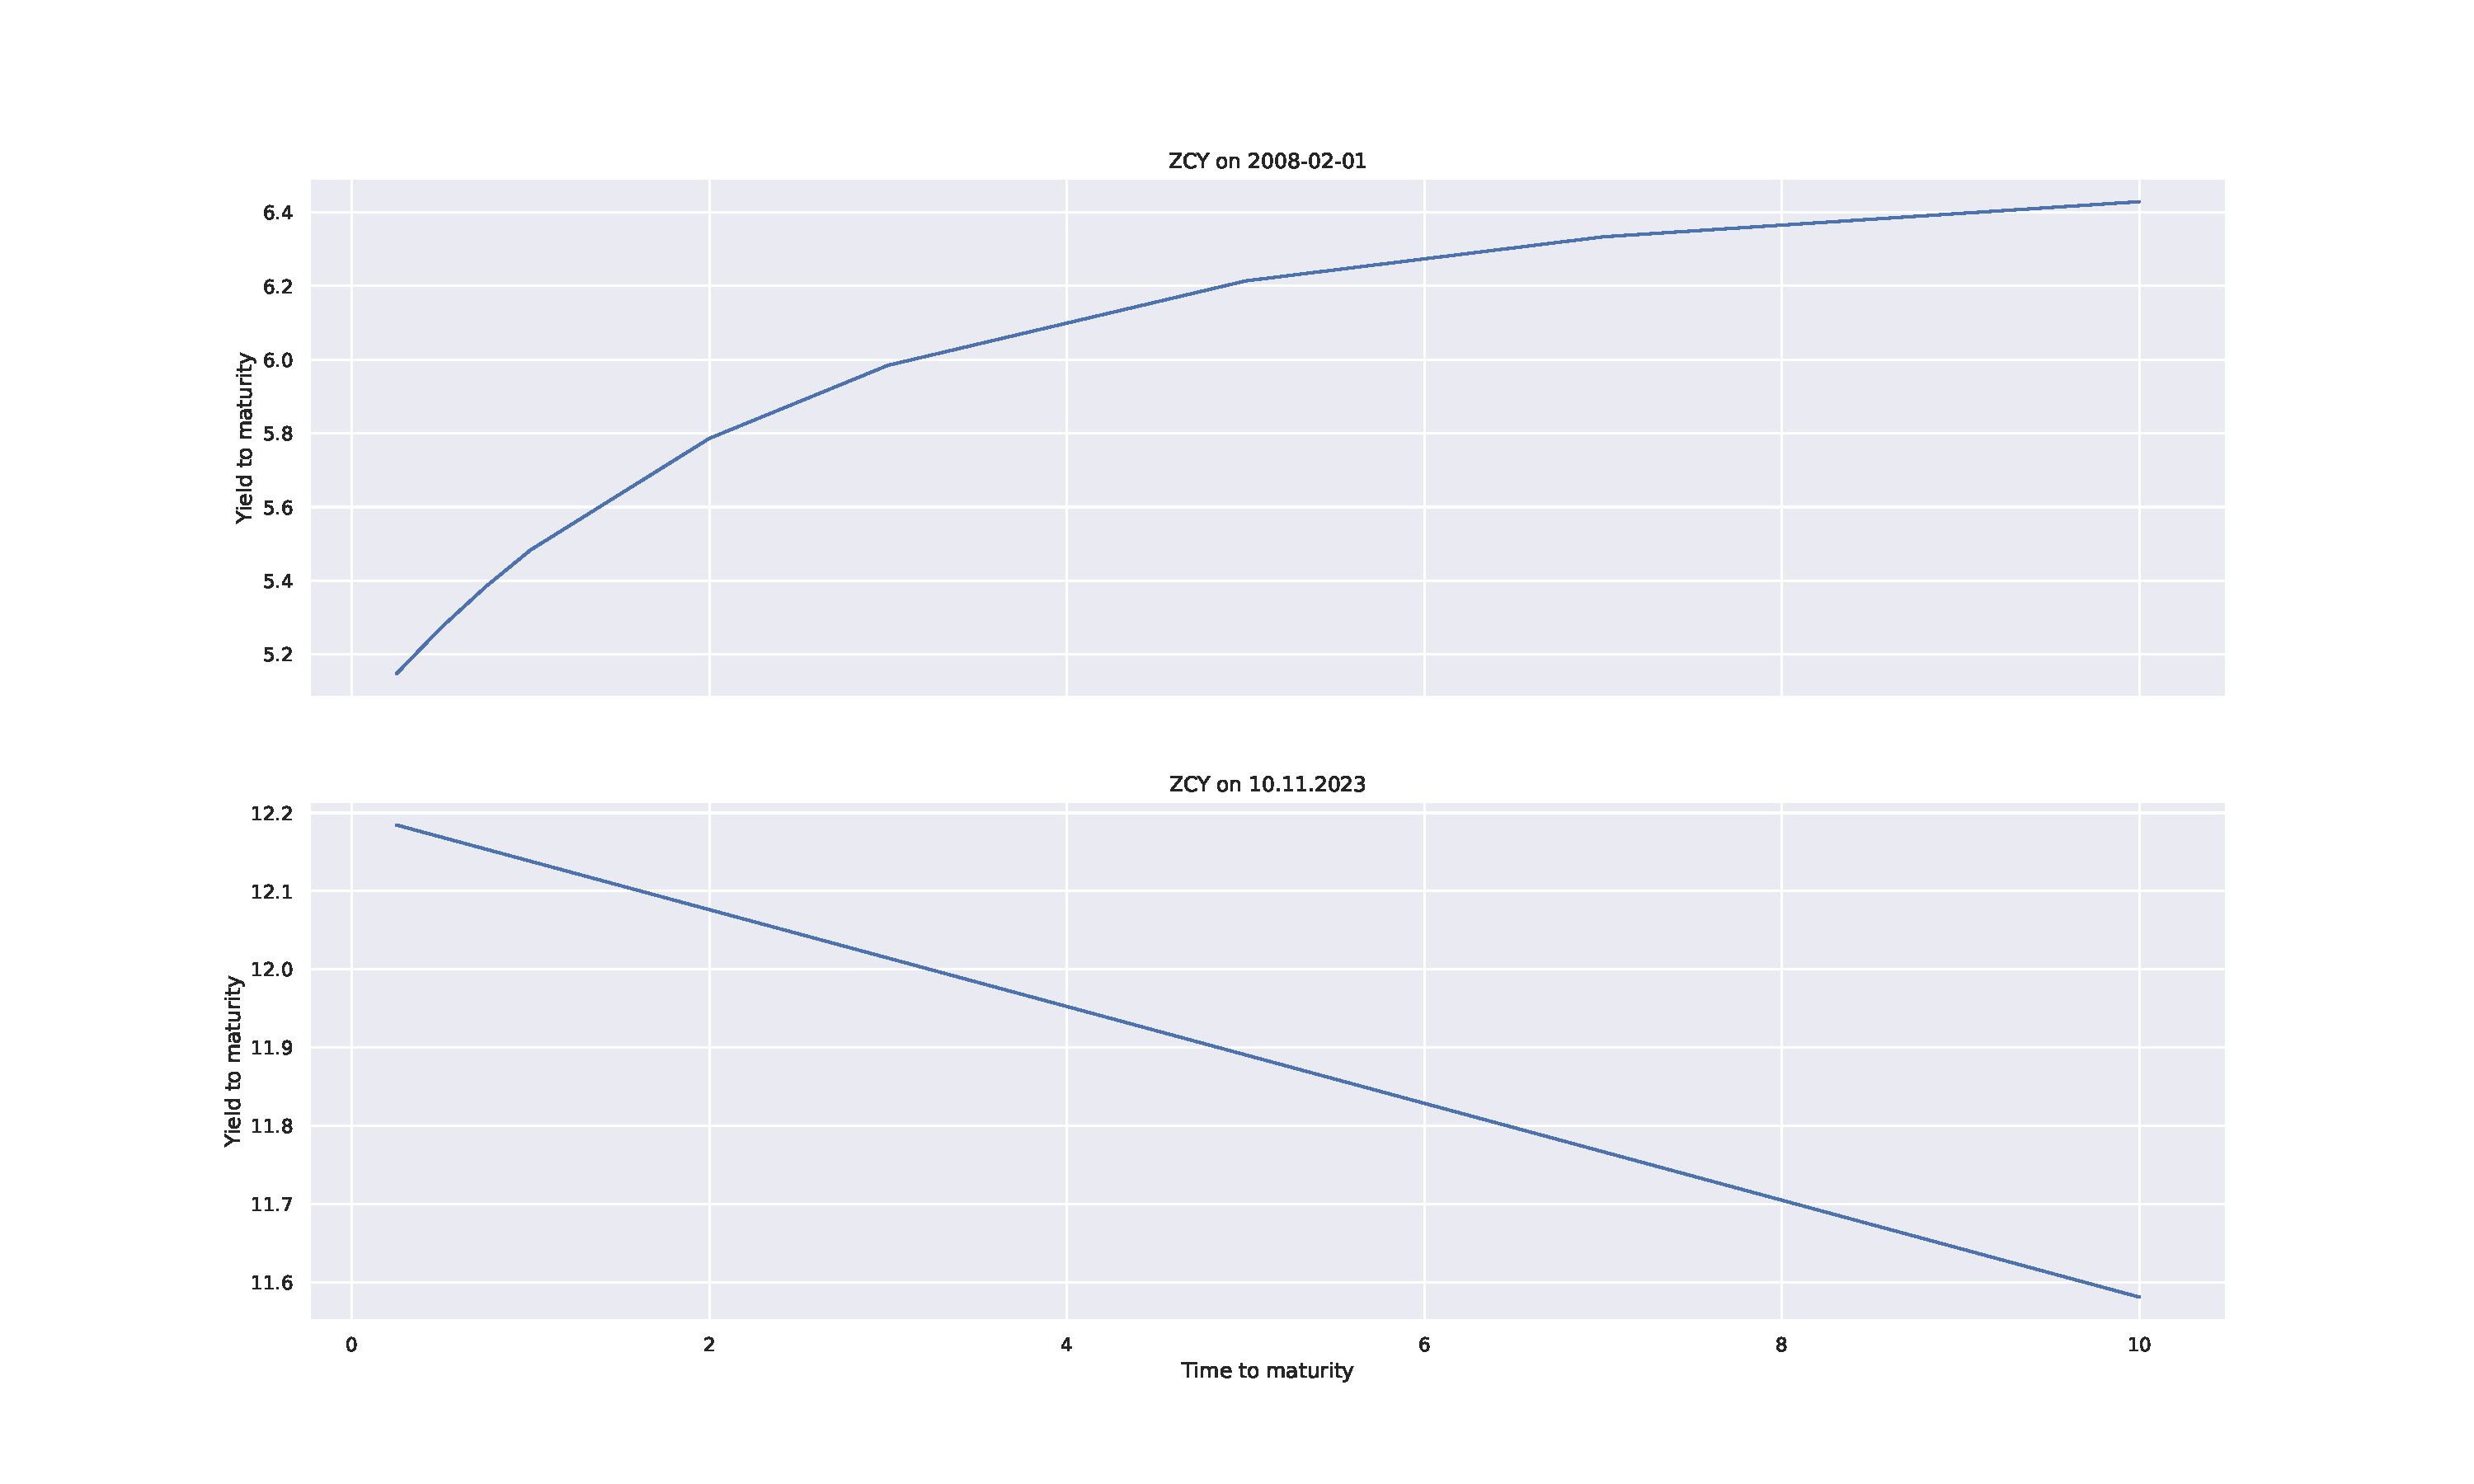
\includegraphics[scale=0.21]{fig/ZCYp.pdf}
            \caption{The yield curves in two different moments of time}
            \label{fig:ZCY}
        \end{figure}
    \end{frame}

    \begin{frame}{The first approach: time series models}
        \begin{table}
            \centering
            \begin{tabular}{|c c c c c c c|} 
                \hline
                Maturity & autoARIMA & ARIMA(0, 0, 0) & RW & VECM(2) & GARCH \\
                \hline
                3m & $0.0045$ & $0.0047$ & $0.0109$ & $0.0193$ & $0.6115$ \\ 
                \hline
                6m & $0.0039$  & 0.$0041$ & $0.0100$ & $0.0182$ & $0.4658$ \\
                \hline
                9m & $0.0035^{**}$ & $0.0038$ & $0.0095$ & $0.0178$ & $0.5676$ \\
                \hline
                12m & $0.0038^{**}$ & $0.0039$ & $0.0069$ & $0.0194$ & $0.7794$ \\
                \hline
                5y & $0.0052$ & $0.0053$ & $0.0072$ & $0.0182$ & $1.2742$\\
                \hline
                15y & $0.0059$ & $0.0061$ & $0.0076$ & $0.0174$ & $1.9276$ \\ 
                \hline
            \end{tabular}
            \caption{}
        \end{table}

    \end{frame}

    \begin{frame}{Nelson-Siegel parametric model}{Model definition}
        The static NS model is defined as follows:
            \begin{equation}\label{eq:NS}
                G(T) = \beta_0 + (\beta_1+\beta_2)\frac{\tau}{T}\left(1-e^{-\frac{T}{\tau}}\right)-\beta_2  e^{-\frac{T}{\tau}},
            \end{equation}
            where $T$ is the time to maturity, $G(T)$ is the yield estimator of the government bonds from the curve basis, 
            and the parameters to be estimated are
            \begin{enumerate}
                \item $\tau$ is the 'typical' time to maturity, 
                \item $\beta_0$ is the long-run of zero-bond yields, 
                \item $\beta_1$ is the mid-run of zero-bond yields, 
                \item $\beta_2$ is the short-run of zero-bond yields.
            \end{enumerate}
    \end{frame}

    \begin{frame}{Nelson-Siegel parametric model}{Forecasting the factors}
    \begin{tabular}{|c | c c c|} 
        \hline
        Coefficient & auto-ARIMA & VAR(1) & RW \\
        \hline
        $\beta_0$ & $53.78356$ & $131.1459$ & $66.3105$ \\ 
        \hline
        $\beta_1$ & $63.31042$ & $143.9235$ & $66.25878$ \\
        \hline
        $\beta_2$ & $133.9688$ & $388.3436$ & $177.1525$ \\
        \hline
        $\tau$ & $1.083687$ & $2.569167$ & $1.328986$ \\
        \hline
    \end{tabular}
\end{frame}

    \begin{frame}{Conclusion and next steps}
    We concluded that:
    \begin{enumerate}
        \item It is better not to use simple time series 
        models to predict bond returns \ldots
        \item \ldots since the first difference of bonds is martingale relative to the filtering of these models.
        \item Research structural breaks.
    \end{enumerate}
    Our plans for the future of this paper:
    \begin{enumerate}
        \item Try the more complicated modifications of NS model.
        \item Add exogeneous variables.
        \item Research the structural breaks.
    \end{enumerate}
    \end{frame}


\end{document}